\section{Implementation and Dataset}\label{secdataset}

We developed our segmentation tool by integrating both \texttt{Stardist} and \texttt{SAM}, using \texttt{Stardist} for nuclei segmentation and a customized version of \texttt{SAM}, which we refer to as \texttt{MyoSAM}, for myotube segmentation. The primary modification in our approach involved training \texttt{MyoSAM} to enhance its capability for precise myotube segmentation. Below, we detail how each model was implemented to meet our project objectives.

\subsection{\texttt{Stardist}}
\texttt{Stardist} exceeded our expectations for nuclei segmentation, eliminating the need for additional training. We employed the ``2D\_versatile\_fluo'' model in its default configuration, which had been trained on a total of 1697 images sourced from three datasets. Two of these datasets are synthetic, designed to simulate extreme scenarios that pose significant challenges in the segmentation of cell nuclei.

\subsection{Data Labeling}

Our project's goal is to provide medical experts specializing in the musculoskeletal domain with a tool to expedite the segmentation of myotubes, a process traditionally known for its complexity. Initially, we faced a catch-22: to train a model for myotube segmentation, we required labeled data, yet obtaining this data necessitated undergoing the very labor-intensive process we aimed to streamline. At the outset, we had no labeled data at our disposal. However, inspired by the promising zero-shot performance of \texttt{SAM}, particularly its ability to recognize myotubes and their shapes, we decided to leverage it to accelerate our data annotation process, despite its tendency to produce extraneous masks. To cautiously generate labeled data suitable for training, our workflow involved several steps:

We developed a tool, that employed the great zero-shot generalization performance of \texttt{SAM}, which enabled our experts to review all predicted masks and discard any inaccuracies. This approach noticeably reduced the time required for data labeling, especially when compared to manual annotation. The myotube images we worked with varied in size, from 4000x4000 pixels to as large as 9000x9000 pixels. Predicting masks on images larger than 2000x2000 pixels demanded substantial computing resources not at our disposal, causing us to adopt an image patching technique for larger images.
Given that \texttt{SAM} was trained on natural images, which differ drastically from the dark, detail-sparse backgrounds of most microscopy images, we allowed our expert to preprocess the images to improve mask prediction accuracy. Our preprocessing efforts revealed that, contrary to our initial belief, myotube microscopy images do not have a purely black background but instead ones with subtle coloring, from the markers used to visualize myotubes and nuclei. By focusing on eliminating large clusters of pixels with identical lightness based on the HSL space, we aimed to isolate the myotubes against a black background, enhancing their visibility. This preprocessing step, along with the expert validation of zero-shot generated masks, markedly accelerated the annotation process.
However, image patches needed to be reassembled into their original dimensions, requiring adjustments to the binary masks to reflect the original image accurately. This reassembly process involved stitching together myotube segments that had been divided across patches. We merged masks at horizontal and vertical divisions, dropping any masks without corresponding segments in adjacent patches and merging those with a considerable overlap as measured by the intersection over union at the edges.
\texttt{SAM}'s design to accommodate prompt ambiguity led to the generation of redundant masks for the same myotube. To address this, we retained only one mask per myotube, discarding any that were completely enclosed by larger ones. Additionally, \texttt{SAM} sometimes produced disconnected masks for a single instance, which were also removed.
The refined predictions were then presented to our expert for final validation and manual completion of the segmentation process. This iterative approach to data annotation was indispensable for creating a high-quality training dataset. Without it, we would have faced serious delays in acquiring manually annotated images diverse enough to train our model effectively. This diversity is crucial to accurately represent the true data distribution of myotube microscopy images in terms of their size, color, shape, and distribution.

\subsection{\texttt{MyoSAM} vs. \texttt{SAM}}
One distinction between \texttt{SAM} and our curated version, \texttt{MyoSAM} stems from our analysis of myotube images and their unique pixel activation patterns. Unlike \texttt{SAM}, which was designed for everyday images with different pixel distributions, \texttt{MyoSAM} required specific normalization for the RGB channels, using mean values of red 13.21, green 21.91, and blue 15.04, and standard deviations of 7.26, 16.40, and 12.12. These values differ from the ones contained in the exploratory analysis in Sec.~\ref{secsam} because they were calculated on both plain and preprocessed images. Additionally, given that myotubes do not possess hierarchical structures of interest, we simplified \texttt{MyoSAM} to use a single prediction head instead of three. We also limited the model to two types of prompts: point prompts to later make use of the AutoMaskGenerator algorithm introduced in the original paper and discussed in Sec.~\ref{SAMbg} and mask prompts which were used to streamline the focus of the model and improving efficiency of training.
A retained feature from \texttt{SAM} is the use of bilinear interpolation to resize input images to a standard size of 1024x1024 for compatibility with the vision transformer. For large images, \texttt{MyoSAM} employs a patching strategy similar to that described in our data labeling process. Each image is divided into patches if necessary, with \texttt{MyoSAM} predicting masks for each patch using the \texttt{SAM} AutomaskGenerator. After segmentation, the patches are reassembled and masks are merged at split points. Finally, we calculate all relevant metrics for the segmented images, providing comprehensive data for medical analysis.

\subsection{\texttt{MyoSAM} Training Approach}
In developing \texttt{MyoSAM}, our training methodology was based on the original \texttt{SAM} training process, with adjustments made to accommodate the challenges of data scarcity and computational resources. This section outlines the key differences and strategies we implemented.
Our dataset comprised 19 annotated myotube images, which we divided into patches of 1500x1500 pixels. This division resulted in a total of 283 patches (cf. Fig.~\ref{figtraindata}). To augment our dataset and increase its diversity, we applied 16 different augmentation techniques to these patches. Specifically, we performed color jittering five times on each patch to make the training set independent of color. In terms of spatial transformations, we applied five random rotations with rotation angles between $\pm 45^{\circ}$, inverted the image, and applied both vertical and horizontal flips. This created a more isotropic dataset. In order to imitate visual distortions, we added Gaussian noise twice, and applied a Gaussian blur. These augmentation processes expanded our dataset to 4528 patches. The primary issue with the data available to us was that nearly half of the patches originated from just three images. This was due to the noteworthy size discrepancy between these images and the other 16, leading to a skewed data distribution and exacerbating the challenge of achieving representative data variability, as illustrated in Fig.~\ref{figtraindata}.

\begin{figure}
	\centering
	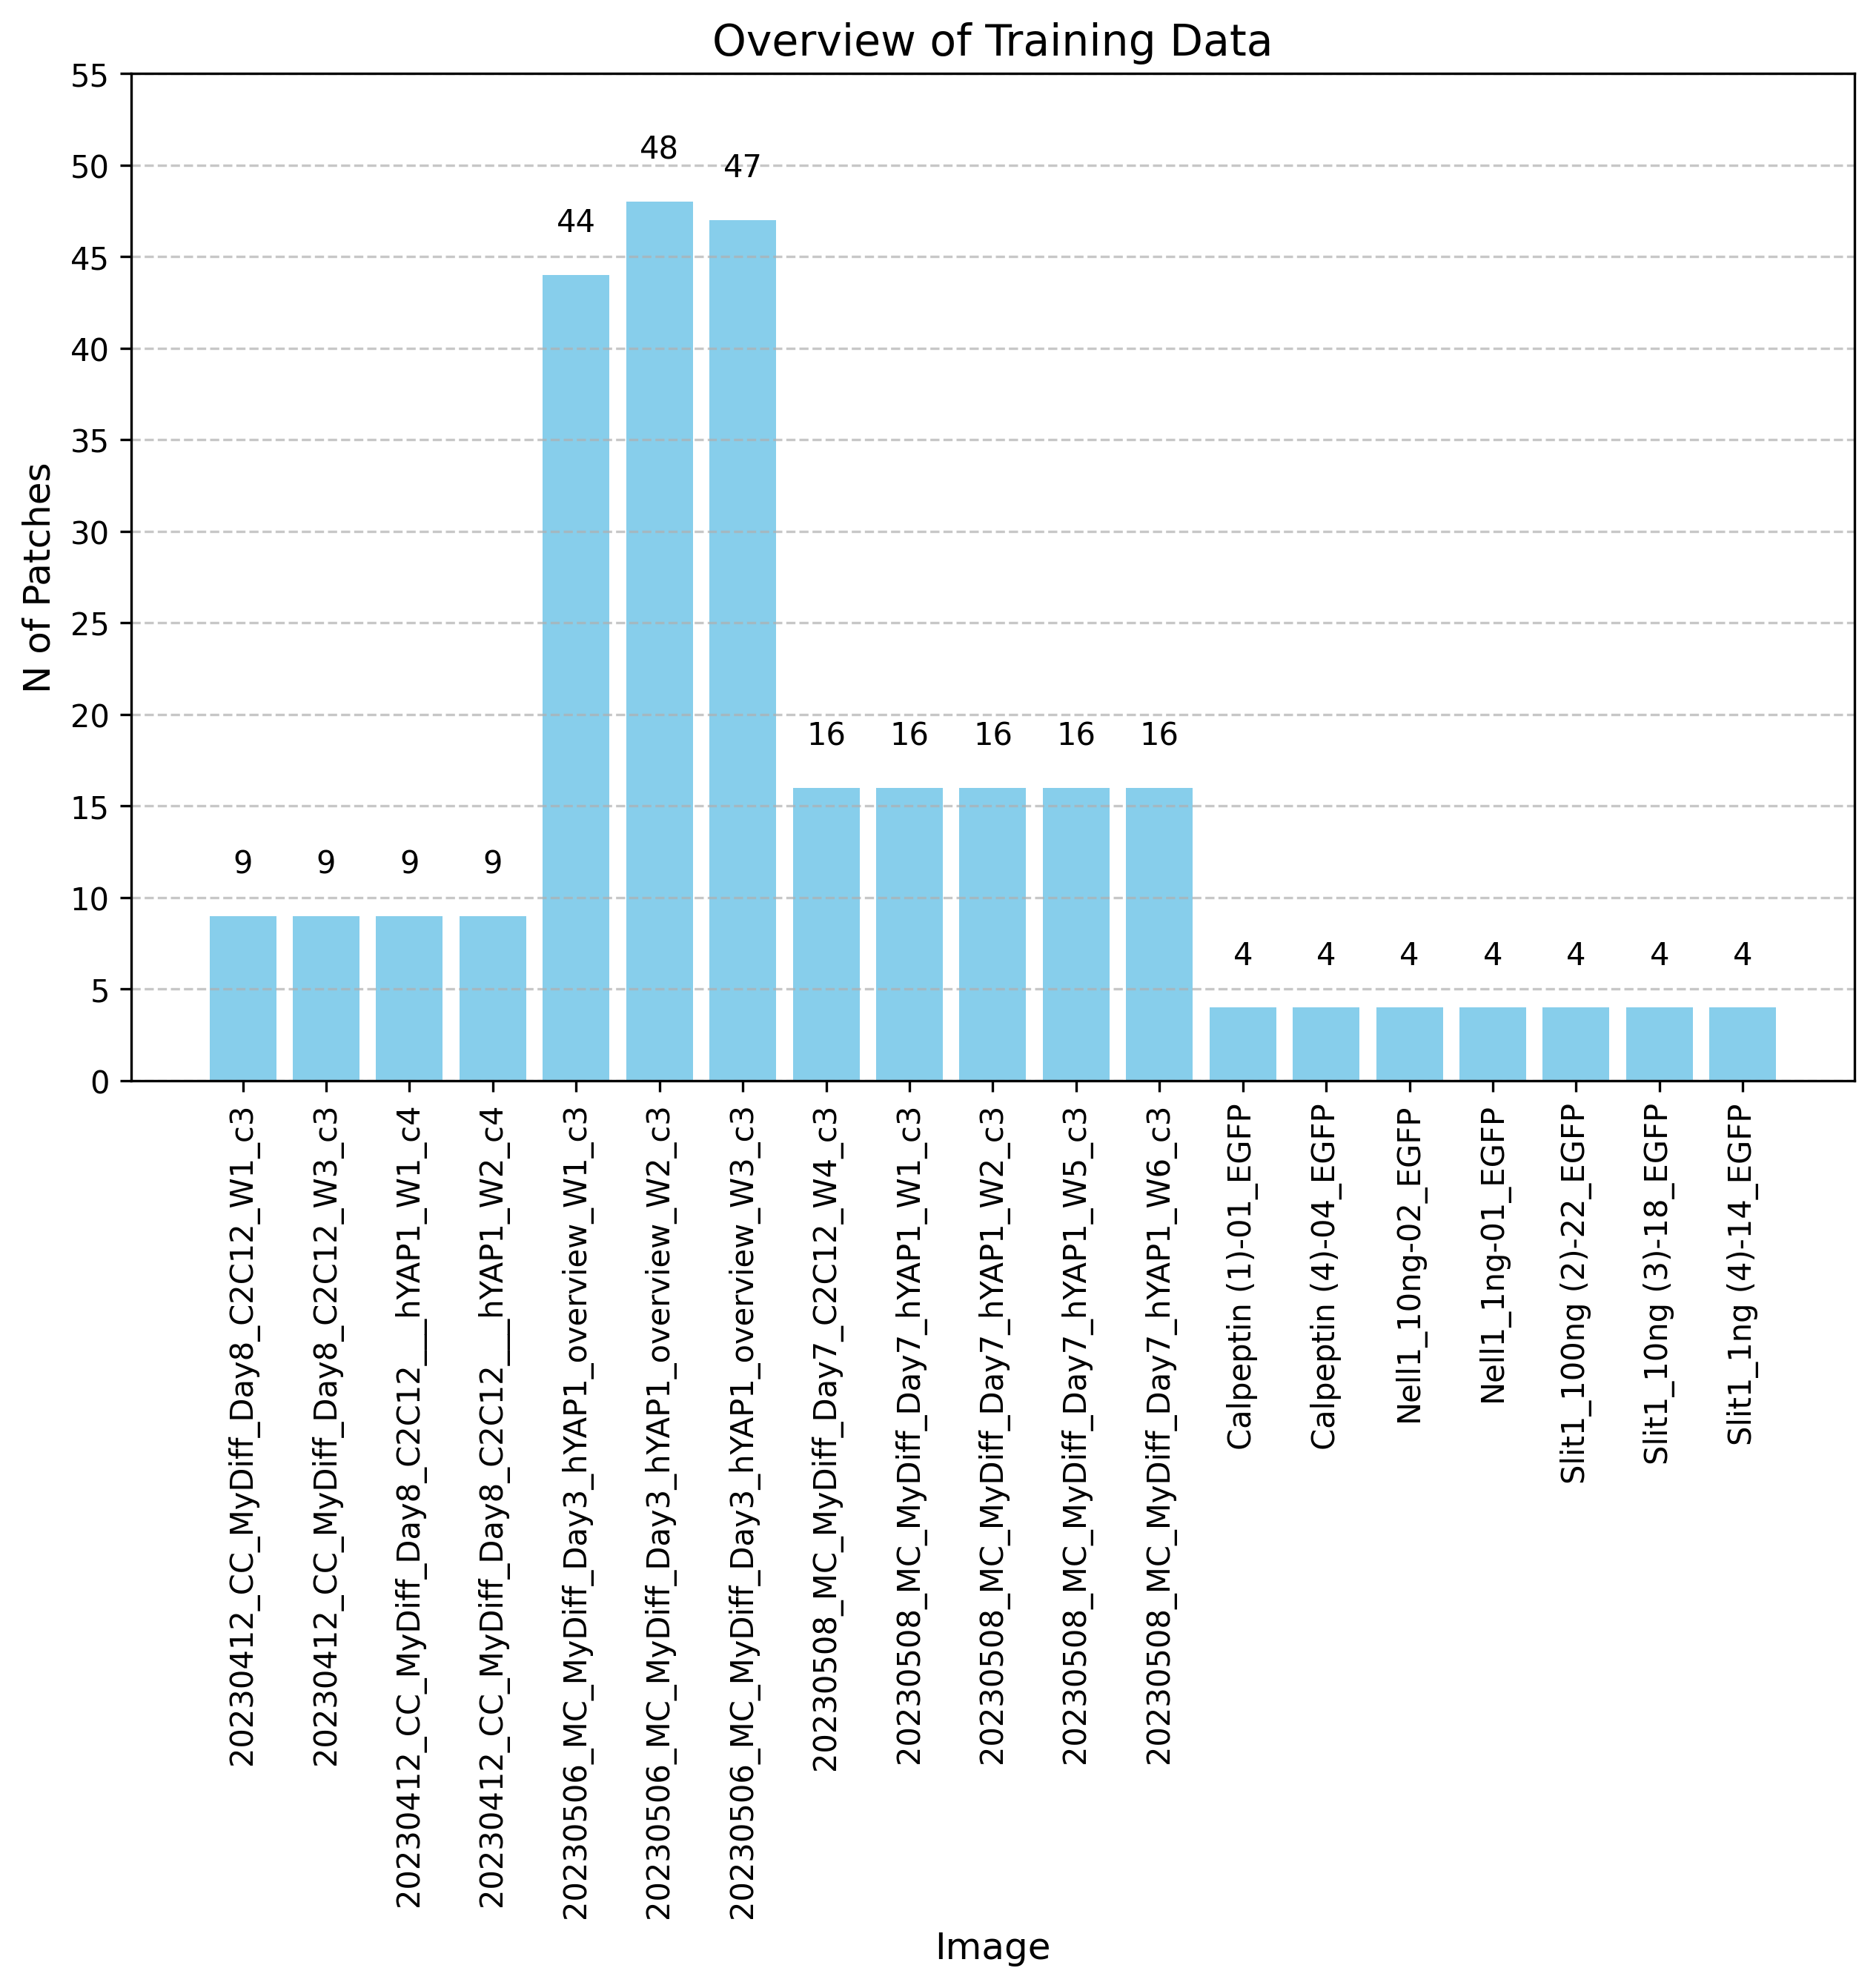
\includegraphics[width=\textwidth]{"images/overview_training_data.png"}
	\caption[Patches per image]{Overview of images and their respective number of patches.}
	\label{figtraindata}
\end{figure}

We divided the augmented dataset into training (80\%) and validation (20\%) sets. To ensure a balanced distribution of images and unbiased estimation of validation error, we shuffled the patches derived from the original images before splitting to make sure that both training and validation sets contain diversified patches and all images are represented in both sets.
During training, we limited the number of instances sampled in each step to 54 in order to maintain stable memory usage and prevent out-of-memory issues. However, for validation purposes, we consistently used the same instances to ensure the comparability of validation error over time. The training was planned for 40 epochs but was terminated at the 21st epoch due to the early stopping criterion of stagnant validation error.
To enhance training efficiency and manage memory use more effectively, we utilized Automated Mixed Precision (AMP) training. Additionally, we adopted Distributed Data Parallel (DDP) training to distribute the computation across six 40GB GPUs, allowing us to parallelize the workload effectively. We used PyTorch \cite{paszke2019pytorch} implementations for both AMP and DDP. The training batches were configured to include six patches, corresponding to one patch per GPU, with each patch containing up to 54 instances. This setup meant that a single training step could involve processing up to 324 instances.
For optimization, we chose the AdamW optimizer with $\beta_1 = 0.9$ and $\beta_2 = 0.999$, incorporated L2 regularization with $\lambda = 0.1$ to prevent overfitting and set an initial learning rate of $10^{-4}$. We also applied a learning rate decay factor of 0.1 after every second epoch to gradually reduce the learning rate and improve convergence (cf. Fig.~\ref{figlr}). The loss functions and training algorithm used in training \texttt{MyoSAM} were consistent with those used in \texttt{SAM}'s original training. The progressions of test and train loss can be found in Fig.~\ref{figtrainloss}-Fig.~\ref{figtraintestloss}.

